% Generated from figures/generated/ch08-geometry.svg; do not hand edit.
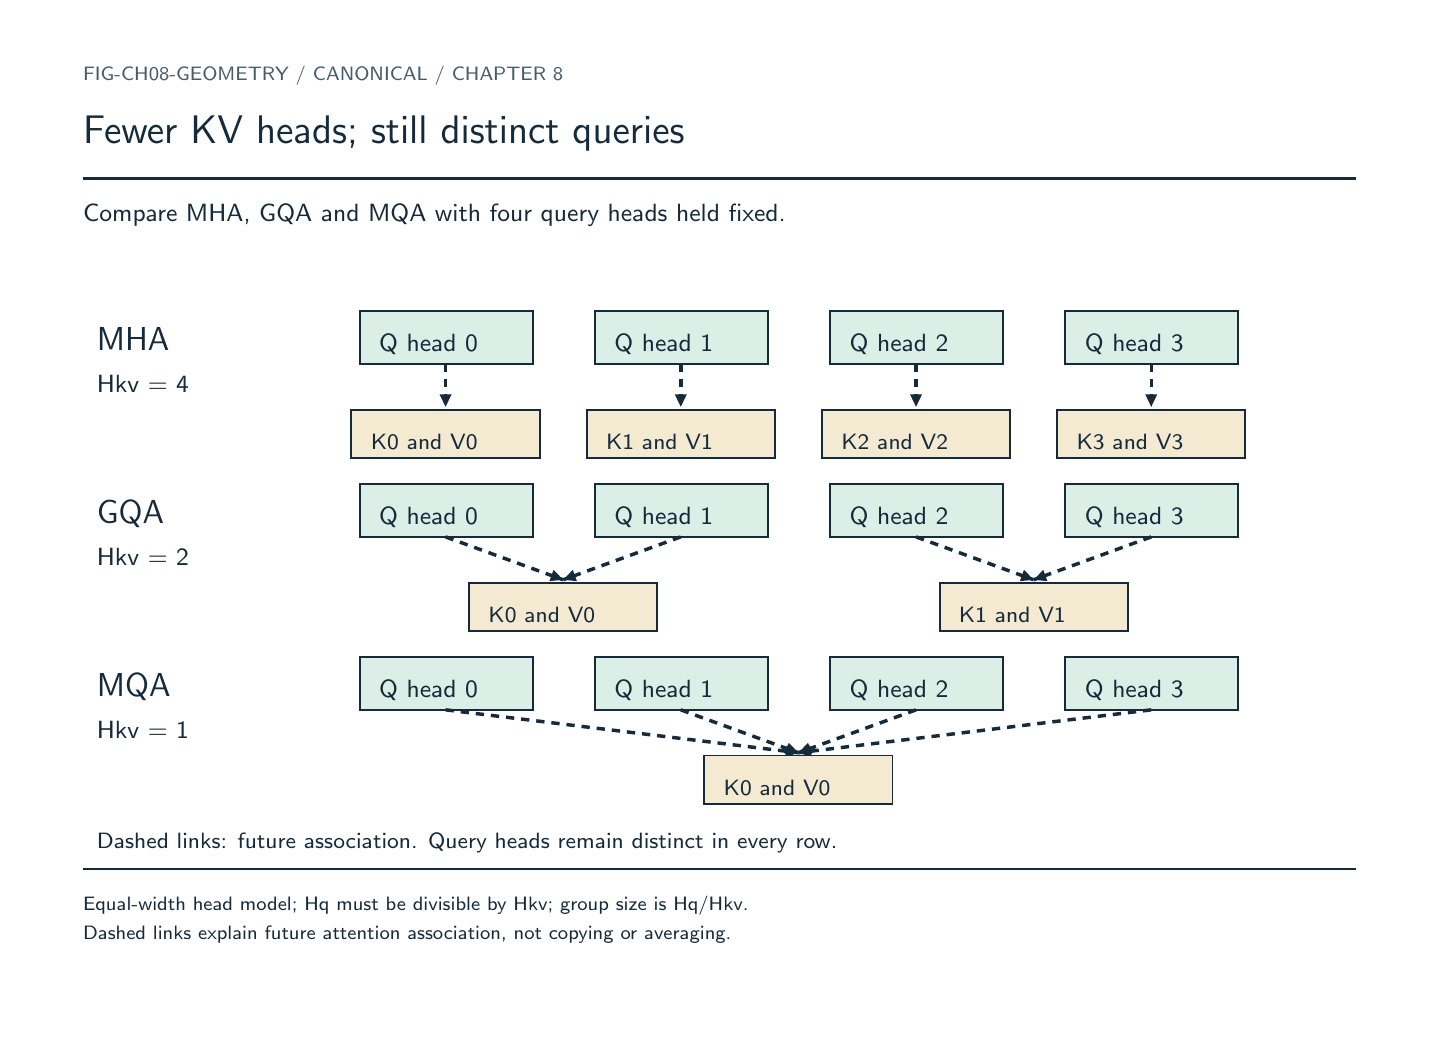
\begin{tikzpicture}[x=.5pt,y=-.5pt]
\path[use as bounding box] (0,0) rectangle (1000,720);
\path[fill=white,draw=none,line width=0.5pt] (0.0,0.0) rectangle (1000.0,720.0);
\node[inner sep=0pt,outer sep=0pt,anchor=base west,text={rgb,255:red,70;green,92;blue,107},font=\sffamily\fontsize{7.0}{8.4}\selectfont] at (40,38) {FIG-CH08-GEOMETRY  /  CANONICAL / CHAPTER 8};
\node[inner sep=0pt,outer sep=0pt,anchor=base west,text={rgb,255:red,21;green,43;blue,60},font=\sffamily\fontsize{15.0}{18.0}\selectfont] at (40,84) {Fewer KV heads; still distinct queries};
\draw[fill=none,draw={rgb,255:red,21;green,43;blue,60},line width=0.75pt] (40,109) -- (960,109);
\node[inner sep=0pt,outer sep=0pt,anchor=base west,text={rgb,255:red,21;green,43;blue,60},font=\sffamily\fontsize{9.5}{11.4}\selectfont] at (40,140) {Compare MHA, GQA and MQA with four query heads held fixed.};
\node[inner sep=0pt,outer sep=0pt,anchor=base west,text={rgb,255:red,21;green,43;blue,60},font=\sffamily\fontsize{11.5}{13.799999999999999}\selectfont] at (50,233) {MHA};
\node[inner sep=0pt,outer sep=0pt,anchor=base west,text={rgb,255:red,21;green,43;blue,60},font=\sffamily\fontsize{9.0}{10.799999999999999}\selectfont] at (50,264) {Hkv = 4};
\path[fill={rgb,255:red,220;green,239;blue,231},draw={rgb,255:red,21;green,43;blue,60},line width=0.7pt] (240.0,205.0) rectangle (365.0,243.0);
\node[inner sep=0pt,outer sep=0pt,anchor=base west,text={rgb,255:red,21;green,43;blue,60},font=\sffamily\fontsize{9.0}{10.799999999999999}\selectfont] at (254,234) {Q head 0};
\path[fill={rgb,255:red,220;green,239;blue,231},draw={rgb,255:red,21;green,43;blue,60},line width=0.7pt] (410.0,205.0) rectangle (535.0,243.0);
\node[inner sep=0pt,outer sep=0pt,anchor=base west,text={rgb,255:red,21;green,43;blue,60},font=\sffamily\fontsize{9.0}{10.799999999999999}\selectfont] at (424,234) {Q head 1};
\path[fill={rgb,255:red,220;green,239;blue,231},draw={rgb,255:red,21;green,43;blue,60},line width=0.7pt] (580.0,205.0) rectangle (705.0,243.0);
\node[inner sep=0pt,outer sep=0pt,anchor=base west,text={rgb,255:red,21;green,43;blue,60},font=\sffamily\fontsize{9.0}{10.799999999999999}\selectfont] at (594,234) {Q head 2};
\path[fill={rgb,255:red,220;green,239;blue,231},draw={rgb,255:red,21;green,43;blue,60},line width=0.7pt] (750.0,205.0) rectangle (875.0,243.0);
\node[inner sep=0pt,outer sep=0pt,anchor=base west,text={rgb,255:red,21;green,43;blue,60},font=\sffamily\fontsize{9.0}{10.799999999999999}\selectfont] at (764,234) {Q head 3};
\draw[fill=none,draw={rgb,255:red,21;green,43;blue,60},line width=1.25pt,dash pattern=on 3.0pt off 2.5pt] (302,243) -- (302.0,274);
\path[fill={rgb,255:red,21;green,43;blue,60},draw=none,line width=0.5pt] (302.00,274.00) -- (297.65,265.00) -- (306.35,265.00) -- cycle;
\path[fill={rgb,255:red,244;green,234;blue,210},draw={rgb,255:red,21;green,43;blue,60},line width=0.7pt] (234.0,276.0) rectangle (370.0,311.0);
\node[inner sep=0pt,outer sep=0pt,anchor=base west,text={rgb,255:red,21;green,43;blue,60},font=\sffamily\fontsize{8.5}{10.2}\selectfont] at (248.0,305) {K0 and V0};
\draw[fill=none,draw={rgb,255:red,21;green,43;blue,60},line width=1.25pt,dash pattern=on 3.0pt off 2.5pt] (472,243) -- (472.0,274);
\path[fill={rgb,255:red,21;green,43;blue,60},draw=none,line width=0.5pt] (472.00,274.00) -- (467.65,265.00) -- (476.35,265.00) -- cycle;
\path[fill={rgb,255:red,244;green,234;blue,210},draw={rgb,255:red,21;green,43;blue,60},line width=0.7pt] (404.0,276.0) rectangle (540.0,311.0);
\node[inner sep=0pt,outer sep=0pt,anchor=base west,text={rgb,255:red,21;green,43;blue,60},font=\sffamily\fontsize{8.5}{10.2}\selectfont] at (418.0,305) {K1 and V1};
\draw[fill=none,draw={rgb,255:red,21;green,43;blue,60},line width=1.25pt,dash pattern=on 3.0pt off 2.5pt] (642,243) -- (642.0,274);
\path[fill={rgb,255:red,21;green,43;blue,60},draw=none,line width=0.5pt] (642.00,274.00) -- (637.65,265.00) -- (646.35,265.00) -- cycle;
\path[fill={rgb,255:red,244;green,234;blue,210},draw={rgb,255:red,21;green,43;blue,60},line width=0.7pt] (574.0,276.0) rectangle (710.0,311.0);
\node[inner sep=0pt,outer sep=0pt,anchor=base west,text={rgb,255:red,21;green,43;blue,60},font=\sffamily\fontsize{8.5}{10.2}\selectfont] at (588.0,305) {K2 and V2};
\draw[fill=none,draw={rgb,255:red,21;green,43;blue,60},line width=1.25pt,dash pattern=on 3.0pt off 2.5pt] (812,243) -- (812.0,274);
\path[fill={rgb,255:red,21;green,43;blue,60},draw=none,line width=0.5pt] (812.00,274.00) -- (807.65,265.00) -- (816.35,265.00) -- cycle;
\path[fill={rgb,255:red,244;green,234;blue,210},draw={rgb,255:red,21;green,43;blue,60},line width=0.7pt] (744.0,276.0) rectangle (880.0,311.0);
\node[inner sep=0pt,outer sep=0pt,anchor=base west,text={rgb,255:red,21;green,43;blue,60},font=\sffamily\fontsize{8.5}{10.2}\selectfont] at (758.0,305) {K3 and V3};
\node[inner sep=0pt,outer sep=0pt,anchor=base west,text={rgb,255:red,21;green,43;blue,60},font=\sffamily\fontsize{11.5}{13.799999999999999}\selectfont] at (50,358) {GQA};
\node[inner sep=0pt,outer sep=0pt,anchor=base west,text={rgb,255:red,21;green,43;blue,60},font=\sffamily\fontsize{9.0}{10.799999999999999}\selectfont] at (50,389) {Hkv = 2};
\path[fill={rgb,255:red,220;green,239;blue,231},draw={rgb,255:red,21;green,43;blue,60},line width=0.7pt] (240.0,330.0) rectangle (365.0,368.0);
\node[inner sep=0pt,outer sep=0pt,anchor=base west,text={rgb,255:red,21;green,43;blue,60},font=\sffamily\fontsize{9.0}{10.799999999999999}\selectfont] at (254,359) {Q head 0};
\path[fill={rgb,255:red,220;green,239;blue,231},draw={rgb,255:red,21;green,43;blue,60},line width=0.7pt] (410.0,330.0) rectangle (535.0,368.0);
\node[inner sep=0pt,outer sep=0pt,anchor=base west,text={rgb,255:red,21;green,43;blue,60},font=\sffamily\fontsize{9.0}{10.799999999999999}\selectfont] at (424,359) {Q head 1};
\path[fill={rgb,255:red,220;green,239;blue,231},draw={rgb,255:red,21;green,43;blue,60},line width=0.7pt] (580.0,330.0) rectangle (705.0,368.0);
\node[inner sep=0pt,outer sep=0pt,anchor=base west,text={rgb,255:red,21;green,43;blue,60},font=\sffamily\fontsize{9.0}{10.799999999999999}\selectfont] at (594,359) {Q head 2};
\path[fill={rgb,255:red,220;green,239;blue,231},draw={rgb,255:red,21;green,43;blue,60},line width=0.7pt] (750.0,330.0) rectangle (875.0,368.0);
\node[inner sep=0pt,outer sep=0pt,anchor=base west,text={rgb,255:red,21;green,43;blue,60},font=\sffamily\fontsize{9.0}{10.799999999999999}\selectfont] at (764,359) {Q head 3};
\draw[fill=none,draw={rgb,255:red,21;green,43;blue,60},line width=1.25pt,dash pattern=on 3.0pt off 2.5pt] (302,368) -- (387.0,399);
\path[fill={rgb,255:red,21;green,43;blue,60},draw=none,line width=0.5pt] (387.00,399.00) -- (377.05,400.00) -- (380.03,391.83) -- cycle;
\draw[fill=none,draw={rgb,255:red,21;green,43;blue,60},line width=1.25pt,dash pattern=on 3.0pt off 2.5pt] (472,368) -- (387.0,399);
\path[fill={rgb,255:red,21;green,43;blue,60},draw=none,line width=0.5pt] (387.00,399.00) -- (393.97,391.83) -- (396.95,400.00) -- cycle;
\path[fill={rgb,255:red,244;green,234;blue,210},draw={rgb,255:red,21;green,43;blue,60},line width=0.7pt] (319.0,401.0) rectangle (455.0,436.0);
\node[inner sep=0pt,outer sep=0pt,anchor=base west,text={rgb,255:red,21;green,43;blue,60},font=\sffamily\fontsize{8.5}{10.2}\selectfont] at (333.0,430) {K0 and V0};
\draw[fill=none,draw={rgb,255:red,21;green,43;blue,60},line width=1.25pt,dash pattern=on 3.0pt off 2.5pt] (642,368) -- (727.0,399);
\path[fill={rgb,255:red,21;green,43;blue,60},draw=none,line width=0.5pt] (727.00,399.00) -- (717.05,400.00) -- (720.03,391.83) -- cycle;
\draw[fill=none,draw={rgb,255:red,21;green,43;blue,60},line width=1.25pt,dash pattern=on 3.0pt off 2.5pt] (812,368) -- (727.0,399);
\path[fill={rgb,255:red,21;green,43;blue,60},draw=none,line width=0.5pt] (727.00,399.00) -- (733.97,391.83) -- (736.95,400.00) -- cycle;
\path[fill={rgb,255:red,244;green,234;blue,210},draw={rgb,255:red,21;green,43;blue,60},line width=0.7pt] (659.0,401.0) rectangle (795.0,436.0);
\node[inner sep=0pt,outer sep=0pt,anchor=base west,text={rgb,255:red,21;green,43;blue,60},font=\sffamily\fontsize{8.5}{10.2}\selectfont] at (673.0,430) {K1 and V1};
\node[inner sep=0pt,outer sep=0pt,anchor=base west,text={rgb,255:red,21;green,43;blue,60},font=\sffamily\fontsize{11.5}{13.799999999999999}\selectfont] at (50,483) {MQA};
\node[inner sep=0pt,outer sep=0pt,anchor=base west,text={rgb,255:red,21;green,43;blue,60},font=\sffamily\fontsize{9.0}{10.799999999999999}\selectfont] at (50,514) {Hkv = 1};
\path[fill={rgb,255:red,220;green,239;blue,231},draw={rgb,255:red,21;green,43;blue,60},line width=0.7pt] (240.0,455.0) rectangle (365.0,493.0);
\node[inner sep=0pt,outer sep=0pt,anchor=base west,text={rgb,255:red,21;green,43;blue,60},font=\sffamily\fontsize{9.0}{10.799999999999999}\selectfont] at (254,484) {Q head 0};
\path[fill={rgb,255:red,220;green,239;blue,231},draw={rgb,255:red,21;green,43;blue,60},line width=0.7pt] (410.0,455.0) rectangle (535.0,493.0);
\node[inner sep=0pt,outer sep=0pt,anchor=base west,text={rgb,255:red,21;green,43;blue,60},font=\sffamily\fontsize{9.0}{10.799999999999999}\selectfont] at (424,484) {Q head 1};
\path[fill={rgb,255:red,220;green,239;blue,231},draw={rgb,255:red,21;green,43;blue,60},line width=0.7pt] (580.0,455.0) rectangle (705.0,493.0);
\node[inner sep=0pt,outer sep=0pt,anchor=base west,text={rgb,255:red,21;green,43;blue,60},font=\sffamily\fontsize{9.0}{10.799999999999999}\selectfont] at (594,484) {Q head 2};
\path[fill={rgb,255:red,220;green,239;blue,231},draw={rgb,255:red,21;green,43;blue,60},line width=0.7pt] (750.0,455.0) rectangle (875.0,493.0);
\node[inner sep=0pt,outer sep=0pt,anchor=base west,text={rgb,255:red,21;green,43;blue,60},font=\sffamily\fontsize{9.0}{10.799999999999999}\selectfont] at (764,484) {Q head 3};
\draw[fill=none,draw={rgb,255:red,21;green,43;blue,60},line width=1.25pt,dash pattern=on 3.0pt off 2.5pt] (302,493) -- (557.0,524);
\path[fill={rgb,255:red,21;green,43;blue,60},draw=none,line width=0.5pt] (557.00,524.00) -- (547.54,527.23) -- (548.59,518.60) -- cycle;
\draw[fill=none,draw={rgb,255:red,21;green,43;blue,60},line width=1.25pt,dash pattern=on 3.0pt off 2.5pt] (472,493) -- (557.0,524);
\path[fill={rgb,255:red,21;green,43;blue,60},draw=none,line width=0.5pt] (557.00,524.00) -- (547.05,525.00) -- (550.03,516.83) -- cycle;
\draw[fill=none,draw={rgb,255:red,21;green,43;blue,60},line width=1.25pt,dash pattern=on 3.0pt off 2.5pt] (642,493) -- (557.0,524);
\path[fill={rgb,255:red,21;green,43;blue,60},draw=none,line width=0.5pt] (557.00,524.00) -- (563.97,516.83) -- (566.95,525.00) -- cycle;
\draw[fill=none,draw={rgb,255:red,21;green,43;blue,60},line width=1.25pt,dash pattern=on 3.0pt off 2.5pt] (812,493) -- (557.0,524);
\path[fill={rgb,255:red,21;green,43;blue,60},draw=none,line width=0.5pt] (557.00,524.00) -- (565.41,518.60) -- (566.46,527.23) -- cycle;
\path[fill={rgb,255:red,244;green,234;blue,210},draw={rgb,255:red,21;green,43;blue,60},line width=0.7pt] (489.0,526.0) rectangle (625.0,561.0);
\node[inner sep=0pt,outer sep=0pt,anchor=base west,text={rgb,255:red,21;green,43;blue,60},font=\sffamily\fontsize{8.5}{10.2}\selectfont] at (503.0,555) {K0 and V0};
\node[inner sep=0pt,outer sep=0pt,anchor=base west,text={rgb,255:red,21;green,43;blue,60},font=\sffamily\fontsize{8.5}{10.2}\selectfont] at (50,593) {Dashed links: future association. Query heads remain distinct in every row.};
\draw[fill=none,draw={rgb,255:red,21;green,43;blue,60},line width=0.75pt] (40,608) -- (960,608);
\node[inner sep=0pt,outer sep=0pt,anchor=base west,text={rgb,255:red,21;green,43;blue,60},font=\sffamily\fontsize{7.5}{9.0}\selectfont] at (40,638) {Equal-width head model; Hq must be divisible by Hkv; group size is Hq/Hkv.};
\node[inner sep=0pt,outer sep=0pt,anchor=base west,text={rgb,255:red,21;green,43;blue,60},font=\sffamily\fontsize{7.5}{9.0}\selectfont] at (40,659) {Dashed links explain future attention association, not copying or averaging.};
\end{tikzpicture}
